\documentclass[a4paper,10pt, notitlepage]{report}
\usepackage[utf8]{inputenc}
\usepackage{natbib}
\usepackage{amssymb}
\usepackage{amsmath}
\usepackage[shortlabels]{enumitem}
\usepackage{xcolor}
\usepackage{url}
\usepackage{cancel}
\usepackage{mathtools}
\usepackage[portuguese]{babel}
\usepackage{newclude}
\usepackage{booktabs}
\usepackage[normalem]{ulem}
\usepackage{listings}
\lstset{
  basicstyle=\ttfamily,
  backgroundcolor=\color{gray!10},
  keywordstyle=\color{green!40!black},
  columns=flexible
}
\usepackage{textcomp}

%%%%%%%%%%%%%%%%%%%% Notation stuff
\newcommand{\pr}{\operatorname{Pr}} %% probability
\newcommand{\vr}{\operatorname{Var}} %% variance
\newcommand{\rs}{X_1, X_2, \ldots, X_n} %%  random sample
\newcommand{\irs}{X_1, X_2, \ldots} %% infinite random sample
\newcommand{\rsd}{x_1, x_2, \ldots, x_n} %%  random sample, realised
\newcommand{\bX}{\boldsymbol{X}} %%  random sample, contracted form (bold)
\newcommand{\bx}{\boldsymbol{x}} %%  random sample, realised, contracted form (bold)
\newcommand{\bT}{\boldsymbol{T}} %%  Statistic, vector form (bold)
\newcommand{\bt}{\boldsymbol{t}} %%  Statistic, realised, vector form (bold)
\newcommand{\emv}{\hat{\theta}}
\DeclarePairedDelimiter\ceil{\lceil}{\rceil}
\DeclarePairedDelimiter\floor{\lfloor}{\rfloor}
\DeclareMathOperator*{\argmax}{arg\,max}
\DeclareMathOperator*{\argmin}{arg\,min}
%%%%
\newif\ifanswers
\answerstrue % comment out to hide answers

% Title Page
\title{Primeira avaliação (A1)}
\author{Disciplina: Modelagem Estatística \\ Instrutor: Luiz Max Carvalho \\ Monitores: Eduardo Adame \& Ezequiel Braga}
\date{15 de abril de 2024}

\begin{document}
\maketitle

\begin{center}
\fbox{\fbox{\parbox{1.0\textwidth}{\textsf{
    \begin{itemize}
        \item O tempo para realização da prova é de 3 horas;
        \item Leia a prova toda com calma antes de começar a responder;
        \item Responda todas as questões sucintamente;
        \item Marque a resposta final claramente com um quadrado, círculo ou figura geométrica de sua preferência;
        \item A prova vale 100 pontos. %A pontuação restante é contada como bônus;
        % \item Apenas tente resolver a questão bônus quando tiver resolvido todo o resto;
        \item Você tem direito a trazer \textbf{\underline{uma} folha de ``cola''} tamanho A4 frente e verso (impressa ou escrita à mão), que deverá ser entregue junto com as respostas da prova.
    \end{itemize}}
}}}
\end{center}
\thispagestyle{empty}
\newpage

\setcounter{page}{1}

% Eu queria alguma historia com o cantor e compositor Crazy Frog

\section*{1. All about that interaction, baby!}

O cantor e compositor Crazy Frog está trabalhando em seu novo álbum, mas está encontrando dificuldades para escrever uma música que seja realmente original e cativante. Para solucionar esse problema, ele contratou uma equipe de estatísticos de primeira linha para ajudá-lo a tomar decisões baseadas em modelos. Entretanto, Crazy Frog faltou às aulas de Modelagem Estatística durante a graduação e precisa de ajuda para interpretar alguns dos diferentes modelos apresentados. Sua tarefa é auxiliar o Frog neste desafio.

Considere o modelo

\begin{equation*}
    Y_i = \beta_0 + \beta_1 X_i + \varepsilon_i,
\end{equation*}
onde $X_1, X_2, \ldots, X_n$ são constantes fixas e $\varepsilon_i$ são variáveis aleatórias independentes e identicamente distribuídas com distribuição $\operatorname{Normal}(0, \sigma^2)$.

Considere agora a seguinte reparametrização:
\begin{equation*}
    Y_i = \alpha_0 + \alpha_1 \cdot (X_i - \bar{X}_n) + \varepsilon_i,
\end{equation*}
onde $\bar{X}_n = n^{-1}\sum_{i=1} X_i$.
Sejam $\widehat{\beta_0}$ e $\widehat{\beta_1}$ os estimadores de máxima verossimilhança (EMVs) para os coeficientes do modelo original e  $\widehat{\alpha_0}$ e $\widehat{\alpha_1}$ os EMVs para os coeficientes do modelo reparametrizado.

\begin{enumerate}[label=\alph*)]
 \item (5 pontos) Mostre que
 \begin{enumerate}
     \item $\widehat{\alpha_0} = n^{-1}\sum_{i=1} Y_i$ e que 
     $ \widehat{\beta_0} \neq \widehat{\alpha_0}$;
     \item $\widehat{\alpha_1} = \widehat{\beta_1}$.
     O que isso significa em termos de interpretação desses coeficientes?
 \end{enumerate}
 \item (10 pontos) Crazy indagou sobre a possibilidade de incluir mais uma das covariáveis que ele consolidou. Portanto, vamos supor agora que temos duas covariáveis contínuas, $X_1$ e $X_2$, e que  o modelo agora é
 \begin{equation*}
     Y_i = \beta_0 + \beta_1 X_{1, i} + \beta_2 X_{2, i} + \beta_3 X_{1, i} X_{2, i} + \varepsilon_i.
 \end{equation*}
 \begin{enumerate}
     \item Descreva em palavras a interpretação de cada coeficiente;
     \item Para $j=1, 2$, defina $m_j = n^{-1}\sum_{i=1}^n X_{j, i}$.
     Considere a transformação $X_{j, i}^{c} = X_{j, i} - m_{j}$  e escreva o modelo
     \begin{equation*}
              Y_i = \beta^{\star}_0 + \beta^{\star}_1 X^{c}_{1, i} + \beta^{\star}_2 X^{c}_{2, i} + \beta^{\star}_3 X^{c}_{1, i} X^{c}_{2, i} + \varepsilon_i.
     \end{equation*}
     A interpretação dos coeficientes mudou? Se sim, como?
 \end{enumerate}
 \item (15 pontos) Uma análise interessante seria mapear os coeficientes do segundo modelo nos coeficientes do primeiro modelo.
 É possível mostrar que 
 \begin{equation*}
     \beta_1 = \beta^{\star}_1 - \beta^{\star}_{3}m_2.
 \end{equation*}
 Encontre as expressões para $\beta_0$, $\beta_2$ e $\beta_3$.
\end{enumerate}
\ifanswers
\include*{A1_2024_sol1}
\fi

\section*{2. \textit{Logito ergo sum}} 

Palmirinha tem recebido muitas reclamações sobre clientes que sentem dor de barriga depois de frequentar sua barraca de pamonha.
Ela suspeita que o que está acontecendo é que a sua pamonha é muito gostosa, e por isso as pessoas comem demais e acabam passando mal.
Assim, ela quer estudar o fenômeno para depois confeccionar uma placa com os dizeres ``Não é aconselhável comer mais que $x^{\star\star}$ gramas de pamonha por dia".
Nesta questão, vamos ajudar Palmirinha a determinar essa quantidade.

Suponha que Palmirinha dispõe de um conjunto de dados que consiste em $n$ observações $Y_i \in \{0, 1\}$, $i = 1, \ldots, n$, onde $Y_i = 1$ se o indivíduo teve dor de barriga e  $Y_i = 0$ caso contrário.
Ela dispõe ainda da quantidade em gramas de pamonha que o $i$-ésimo indivíduo consumiu, $X_i$.

Ela escolhe começar sua modelagem com 
\begin{equation}
\label{eq:bern}
    Y_i \mid X_i \sim \operatorname{Bernoulli}(\theta(X_i)),
\end{equation}
mas ainda está em dúvida sobre como especificar a média condicional $\theta(X_i)$.

Ela considera dois modelos lineares generalizados:
\begin{align*}
    \text{Logit}:\quad & \theta(X_i) = \frac{\exp\left(\beta_0 + \beta_1 X_i\right)}{1 + \exp\left(\beta_0 + \beta_1 X_i\right)}, \\
    \text{Probit}: \quad & \theta(X_i) = \Phi\left(\beta_0 + \beta_1 X_i\right),
\end{align*}
onde $\Phi(x) = (2\pi)^{-1}\int_{-\infty}^x \exp(-t^2/2)\,dt$ é a função de distribuição acumulada (f.d.a. ou c.d.f.) de uma normal padrão.

Palmirinha ajustou os dois modelos a $n=100$ observações e produziu a Figura~\ref{fig:dor_pamonha}.
\begin{figure}[ht]
    \centering
    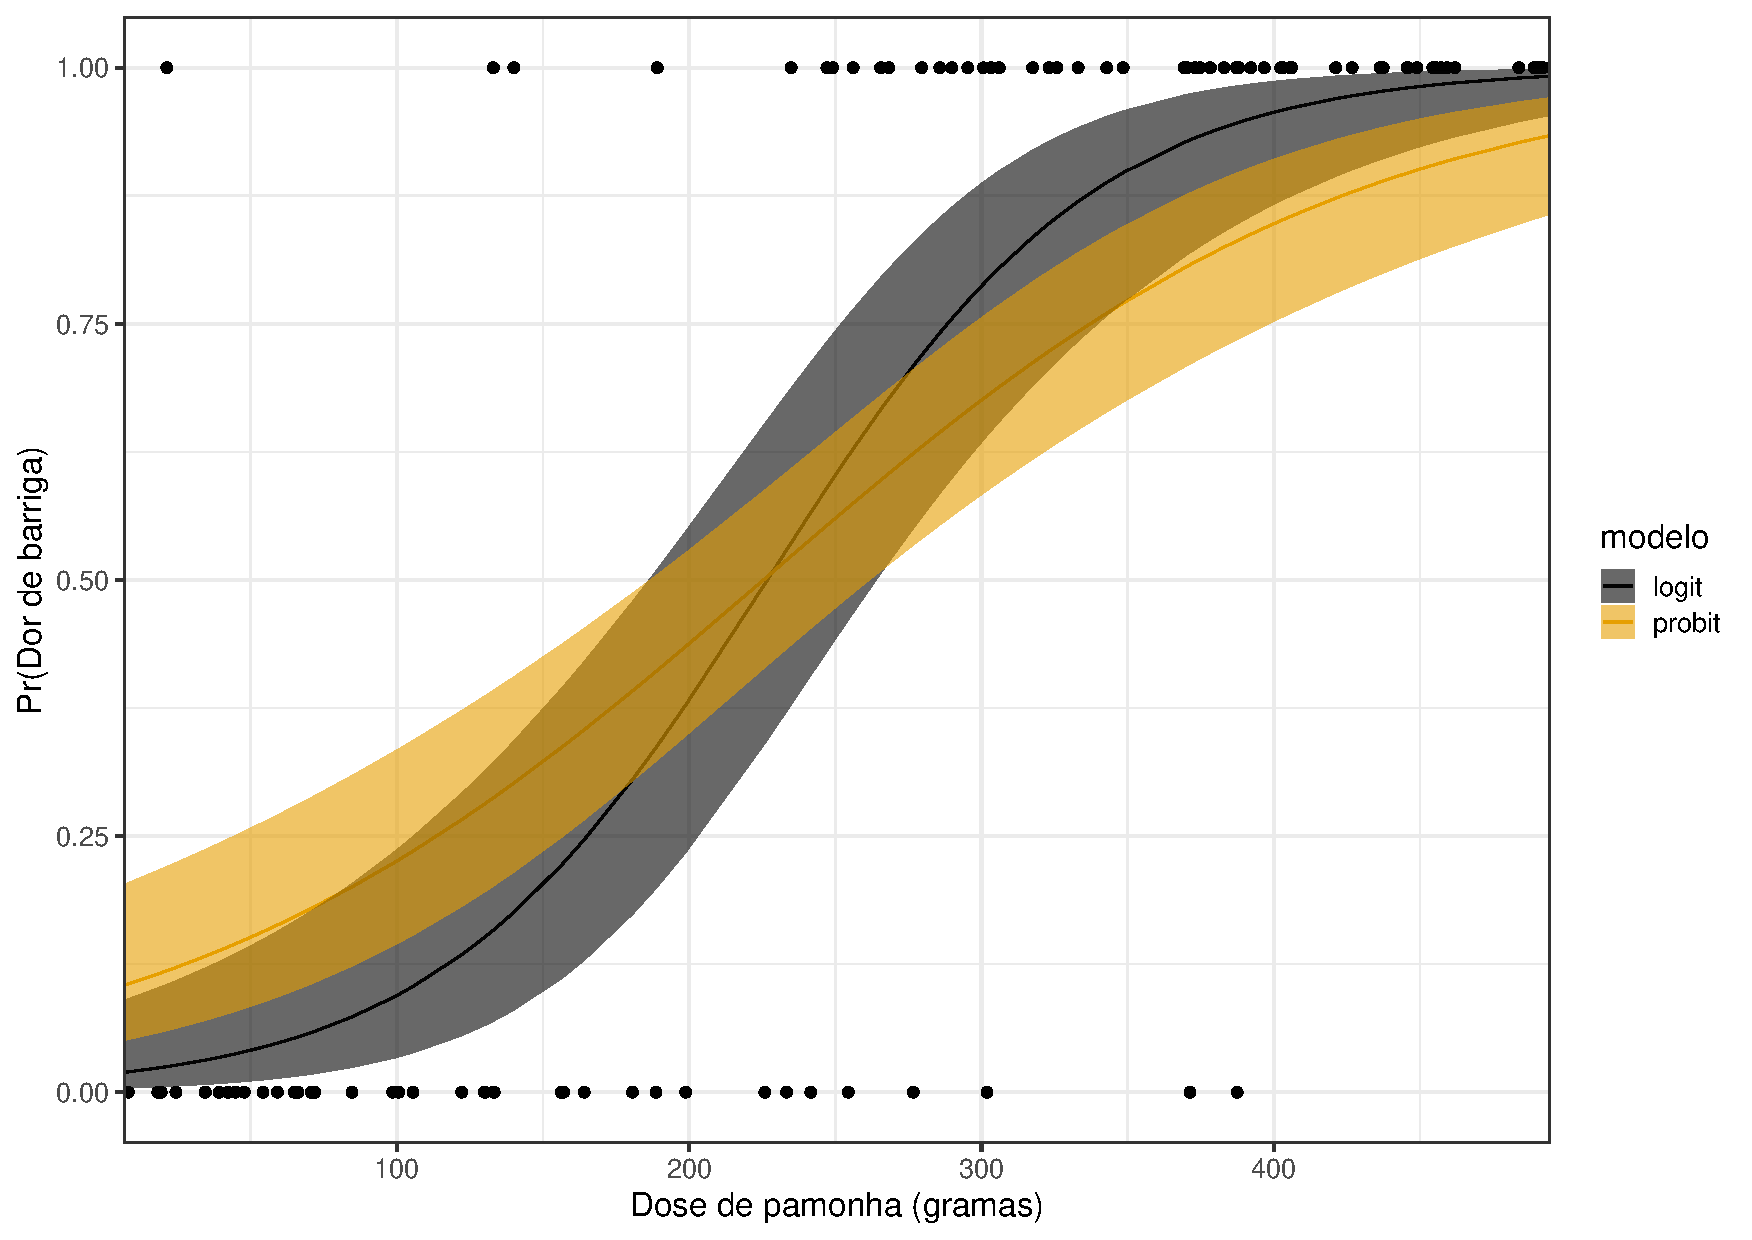
\includegraphics[scale=0.4]{figuras/palmirinha_dor.pdf}
    \caption{Dor de barriga \textit{vs} quantidade de pamonha consumida. Pontos pretos mostram os dados coletados. Linhas coloridas mostram a predição no espaço da probabilidade e as bandas mostram o intervalo de predição de 95\%.}
    \label{fig:dor_pamonha}
\end{figure}
Já o output do R (resumido) ficou assim:
\begin{center}
\begin{lstlisting}[language=R]
> summary(fit.logit)
Call:
glm(formula = Ys ~ doses, family = binomial("logit"))
Coefficients:
             Estimate Std. Error z value Pr(>|z|)    
(Intercept) -4.044785   0.841447  -4.807 1.53e-06 ***
doses        0.017837   0.003259   5.474 4.40e-08 ***

> summary(fit.probit)
Call:
glm(formula = Ys ~ doses, family = binomial("probit"))
Coefficients:
             Estimate Std. Error z value Pr(>|z|)    
(Intercept) -2.216496   0.408629  -5.424 5.82e-08 ***
doses        0.009833   0.001551   6.338 2.32e-10 ***
\end{lstlisting}    
\end{center}
% \begin{itemize}
%     \item logit and probit (done)
%     \item LDp (LD50 como caso especial)
%     \item Mostrar a diferença nas estimativas
%     \item mostrar output do R
%     \item (Na solução): mostrar os betas e a LD50 quando os dois modelos são ajustados sob dois DGPs diferentes.
% \end{itemize}

\begin{enumerate}[label=\alph*)] 
 \item (10 pontos) Mostre que o modelo em (\ref{eq:bern}) pertence à família exponencial canônica.
  \item (20 pontos) Considere $\theta_{\text{logit}}(x) = \frac{\exp\left(\beta_0 + \beta_1 x\right)}{1 + \exp\left(\beta_0 + \beta_1 x\right)}$ e $\theta_{\text{probit}}(x) = \Phi(\beta_0 + \beta_1 x)$. Vamos encará-los como curvas de probabilidades. 
  \begin{enumerate}[i.]
      \item  Exiba $\theta^{\prime}(x) := \frac{\partial}{\partial x}\theta(x)$ para cada um dos modelos acima.
      
      \textbf{Dica}: Note que no nosso caso, o inverso da função de ligação $g^{-1}$ pode ser interpretado como a c.d.f. de uma distribuição contínua e simétrica. 
      Aplique a regra da cadeia.
      \item   Uma quantidade importante é $x^{\star}$ tal que $\theta(x^{\star}) = 1/2$.
      Como os dois modelos serão ajustados no mesmo conjunto de dados, esperamos que $\theta_{\text{logit}}^{\prime}(x^{\star}) \approx \theta_{\text{probit}}^{\prime}(x^{\star})$.
     Sob essa premissa, podemos computar
      \begin{equation*}
          \frac{\hat{\beta_1}^{\text{logit}}}{\hat{\beta_1}^{\text{probit}}} \approx a.
      \end{equation*}
      Determine o valor (aproximado) de $a$ e veja se ele está de acordo com os resultados empíricos obtidos por Palmirinha.
  \end{enumerate}
  \item (10 pontos) Suponha que Palmirinha quer computar $x^{\star\star}$ de modo que $\theta(x^{\star\star}) = 0,8$, isto é, ela quer determinar a dose que faz com que 80\% daqueles que comem $x^{\star\star}$ gramas de pamonha ou mais terem dor de barriga.
  Mostre a Palmirinha como computar essa quantidade sob cada um dos modelos.
 % \textbf{Dica:} 
\end{enumerate} 
\ifanswers
\include*{A1_2024_sol2}
\fi

\section*{3. Your AIC ain't that big...}

A comparação de modelos é uma das principais preocupações da Estatística aplicada. 
Para um modelo paramétrico $\mathcal{M}$ qualquer, o \textit{Akaike Information Criterion} (AIC) é dado por
\begin{equation*}
    \operatorname{AIC}_{\mathcal{M}} = 2k - 2\log(\hat{L}),
\end{equation*}
onde $k$ é número de parâmetros de $\mathcal{M}$ e $\hat{L} = f(\boldsymbol{z} ; \hat{\theta})$ é a verossimilhança avaliada no estimador de máxima verossimilhança dos parâmetros $\theta$, $\hat{\theta}$.

Tome $ \boldsymbol{X}$ uma matriz real $n \times P$ e $\boldsymbol{Y} = \{Y_1, \ldots, Y_n\}^T \in \mathbb{R}^n$ um vetor contendo os valores da variável dependente.
Considere o modelo 
\begin{equation*}
    E[Y_i] =: \mu_i(\boldsymbol{\beta}) = \boldsymbol{X}_i\boldsymbol{\beta},
\end{equation*}
onde $\boldsymbol{\beta} \in \mathbb{R}^{P}$ é o vetor de coeficientes e parâmetro de interesse.
Para completar a especificação do modelo, vamos assumir que os erros em torno da média condicional (preditor linear) são normalmente distribuídos com variância comum:
\begin{align*}
    Y_i &= \mu_i(\boldsymbol{\beta}) + \varepsilon_i\\
    \varepsilon_i &\overset{\text{i.i.d.}}{\sim}  \operatorname{Normal}(0, \sigma^2),
\end{align*}
com $\sigma^2 \in \mathbb{R}_+$ desconhecida.

\begin{enumerate}[label=\alph*)]
 \item (10 pontos) Exiba a expressão do AIC para um modelo linear com $P$ coeficientes, que vamos chamar de modelo $\mathcal{M}_1$.
 \item (10 pontos)  Suponha agora que  temos um conjunto de   covariáveis que inclui as $P$ do item anterior e mais $Q$ covariáveis.
 Chamemos este modelo de $\mathcal{M}_2$.
 Mostre que
 \begin{equation*}
     \operatorname{AIC}_{\mathcal{M}_2} < \operatorname{AIC}_{\mathcal{M}_1} \iff \frac{\text{SSE}_2}{\text{SSE}_1} < \exp\left(-2Q/n\right),
 \end{equation*}
 onde $\text{SSE}_i$ é a soma de erros quadráticos do modelo $\mathcal{M}_i$.
 \item (10 pontos) Uma quantidade importante na avaliação de modelos lineares é o coeficiente de determinação, $R^2$.
 Mostre que 
  \begin{equation*}
     \operatorname{AIC}_{\mathcal{M}_2} < \operatorname{AIC}_{\mathcal{M}_1} \iff R_{2}^2 - R_{1}^2 > \left(1 - \exp\left(-2Q/n\right)\right) \frac{\text{SSE}_1}{\text{SSE}_0},
 \end{equation*}
 onde $\text{SSE}_0$ é a soma dos erros quadráticos de um modelo só com intercepto.
 \end{enumerate}

\ifanswers
\include*{A1_2024_sol3}
\fi

% \bibliographystyle{apalike}
% \bibliography{refs}

\end{document}          
